
{\normalsize
 \begin{center}                                                                            
 \begin{table}[h!]\label{t2}                                                               
 \centering
 \caption{\footnotesize C\'alculos hechos con dos DFT para ser comparados con los datos
  BCL}                                                                  
 \begin{tabular}{c|ccc}\hline\hline                                                          
 LnDFTBase    & $\langle r_{Ln-O}\rangle$ & $\Delta_{\textnormal{hyd}}\tn{H}$ 
 & $\Delta_{\textnormal{hyd}}\tn{H}_{cp}$ \\ \hline                                               
La1+0B3P86VQZ & 2.2965 & -404.427081 & -404.102876 \\
La1+0TPSShVQZ & 2.3064 & -401.859492 & -400.928329 \\
Ce1+0B3P86VQZ & 2.2761 & -374.249702 & -373.721492 \\
Ce1+0TPSShVQZ & 2.2864 & -373.996352 & -373.430462 \\
Lu1+0B3P86VQZ & 2.093  & -511.468829 & -511.196175 \\
Lu1+0TPSShVQZ & 2.1039 & -509.252533 & -508.744010 \\
 \hline \end{tabular}\end{table}                                                           
 \end{center}                                                                              
}
 \begin{center}                                                                            
 \begin{table}[h!]
 \centering
 \caption{\footnotesize C\'alculos BCL para el sistema de La$^{3+}$ y 
una mol\'ecula agua, usando el el pseudo potencial de 28 electrones 
de Stuttgart y la correspondiente base para La y las bases AUG-cc-pViZ
(i=D, T, Q y 5) para la mo\'ecula de agua.}                                                                  
 \begin{tabular}{c|ccc}\hline\hline                                                          
 Sistema & $\langle r_{Ln-O}\rangle$ & $\Delta_{\textnormal{hyd}}\tn{H}$ 
 & $\Delta_{\textnormal{hyd}}\tn{H}_{cp}$ \\ \hline                                               
La1+0MP2CaoDZ & 2.2958 & -396.35664 & -388.76668 \\
La1+0MP2CaoTZ & 2.2867 & -398.51879 & -394.17115 \\
La1+0MP2CaoQZ & 2.2802 & -401.72554 & -397.57012 \\
La1+0MP2Cao5Z & 2.2745 & -405.37835 & -397.97437 \\
 \hline \end{tabular}\label{tLaCao} 
 \end{table}                                                           
 \end{center}                                                                              

%%%%%%%%%%%%%%%%%%%%%%%%%%%%%%%%%%%%%%%%%%%%%%%%%%5555
\begin{figure}[h]
\centering
\includegraphics[height=8cm,angle=-90]{../Tablas/laCdist.ps}
\caption{\small{Gr\'afica de los datos de la tabla \ref{tLaCao},
distancia del Lantano al ox\'igeno, en funci\'on del tama\~no
de la base de la mol\'ecula de agua.}}
\label{fLaCD}
\end{figure}
%%%%%%%%%%%%%%%%%%%%%%%%%%%%%%%%%%%%%%%%%%%%%%%%%%%%%%
%%%%%%%%%%%%%%%%%%%%%%%%%%%%%%%%%%%%%%%%%%%%%%%%%%5555
\begin{figure}[h]
\centering
\includegraphics[height=8cm,angle=-90]{../Tablas/laCeneh.ps}
\caption{\small{Gr\'afica de los datos de la tabla \ref{tLaCao},
energ\'ia de hitrataci\'on del Lantano, en funci\'on del tama\~no
de la base de la mol\'ecula del agua.}}
\label{fLaCE}
\end{figure}
%%%%%%%%%%%%%%%%%%%%%%%%%%%%%%%%%%%%%%%%%%%%%%%%%%%%%%
 \begin{center}                                                                            
 \begin{table}[h!]
 \centering
 \caption{\footnotesize C\'alculos BCL para el sistema de Lu$^{3+}$ y 
una mol\'ecula agua, usando el el pseudo potencial de 28 electrones 
de Stuttgart y la correspondiente base para Lu y las bases AUG-cc-pViZ
(i=D, T, Q y 5) para la mo\'ecula de agua.}                                                                  
 \begin{tabular}{c|ccc}\hline\hline                                                          
 Sistema & $\langle r_{Ln-O}\rangle$ & $\Delta_{\textnormal{hyd}}\tn{H}$ 
 & $\Delta_{\textnormal{hyd}}\tn{H}_{cp}$ \\ \hline                                               
Lu1+0MP2CaoDZ & 2.0715 & -516.81044 & -506.30335 \\
Lu1+0MP2CaoTZ & 2.0658 & -520.04478 & -512.23601 \\
Lu1+0MP2CaoQZ & 2.0551 & -525.39512 & -514.69588 \\
Lu1+0MP2Cao5Z & 2.0402 & -532.78832 & -516.18853 \\
 \hline \end{tabular}\label{tLuCao}    
 \end{table}                                                           
 \end{center}                                                                              

%%%%%%%%%%%%%%%%%%%%%%%%%%%%%%%%%%%%%%%%%%%%%%%%%%5555
\begin{figure}[h]
\centering
\includegraphics[height=8cm,angle=-90]{../Tablas/luCdist.ps}
\caption{\small{Gr\'afica de los datos de la tabla \ref{tLuCao},
distancia del Lutecio al ox\'igeno, en funci\'on del tama\~no
de la base de la mol\'ecula de agua.}}
\label{fLuCD}
\end{figure}
%%%%%%%%%%%%%%%%%%%%%%%%%%%%%%%%%%%%%%%%%%%%%%%%%%%%%%
%%%%%%%%%%%%%%%%%%%%%%%%%%%%%%%%%%%%%%%%%%%%%%%%%%5555
\begin{figure}[h]
\centering
\includegraphics[height=8cm,angle=-90]{../Tablas/luCeneh.ps}
\caption{\small{Gr\'afica de los datos de la tabla \ref{tLuCao},
energ\'ia de hitrataci\'on del Lutecio, en funci\'on del tama\~no
de la base de la mol\'ecula del agua.}}
\label{fLuCE}
\end{figure}
%%%%%%%%%%%%%%%%%%%%%%%%%%%%%%%%%%%%%%%%%%%%%%%%%%%%%%
 \begin{center}                                                                            
 \begin{table}[h!]
 \centering
 \caption{\footnotesize C\'alculos BCL para el sistema de La$^{3+}$ y 
una mol\'ecula agua, usando el el pseudo potencial de 28 electrones 
de Stuttgart y la correspondiente base para La, el pseudopotencial
de Stuttgart para el ox\'igeno y las bases AUG-cc-pViZ (i=D, T, Q y 5) 
para el hidr\'ogeno.}                                                                  
 \begin{tabular}{c|ccc}\hline\hline                                                          
 Sistema & $\langle r_{Ln-O}\rangle$ & $\Delta_{\textnormal{hyd}}\tn{H}$ 
 & $\Delta_{\textnormal{hyd}}\tn{H}_{cp}$ \\ \hline                                               
La1+0MP2CaBeDZ & 2.2982 & -401.35549 & -388.37423 \\
La1+0MP2CaBeTZ & 2.3154 & -387.60339 & -379.14067 \\
La1+0MP2CaBeQZ & 2.3186 & -382.93170 & -376.29999 \\
La1+0MP2CaBe5Z & 2.3176 & -382.21094 & -376.33214 \\
 \hline \end{tabular}\label{tLaCB}      
 \end{table}                                                           
 \end{center}                                                                              

%%%%%%%%%%%%%%%%%%%%%%%%%%%%%%%%%%%%%%%%%%%%%%%%%%5555
\begin{figure}[h]
\centering
\includegraphics[height=8cm,angle=-90]{../Tablas/laCBdist.ps}
\caption{\small{Gr\'afica de los datos de la tabla \ref{tLaCB},
distancia del Lantano al ox\'igeno, en funci\'on del tama\~no
de la base del hidr\'ogeno.}}
\label{fLaCBD}
\end{figure}
%%%%%%%%%%%%%%%%%%%%%%%%%%%%%%%%%%%%%%%%%%%%%%%%%%%%%%
%%%%%%%%%%%%%%%%%%%%%%%%%%%%%%%%%%%%%%%%%%%%%%%%%%5555
\begin{figure}[h]
\centering
\includegraphics[height=8cm,angle=-90]{../Tablas/laCBeneh.ps}
\caption{\small{Gr\'afica de los datos de la tabla \ref{tLaCB},
energ\'ia de hitrataci\'on del Lantano, en funci\'on del tama\~no
de la base del hidr\'ogeno.}}
\label{fLaCBE}
\end{figure}
%%%%%%%%%%%%%%%%%%%%%%%%%%%%%%%%%%%%%%%%%%%%%%%%%%%%%%
 \begin{center}                                                                            
 \begin{table}[h!]
 \centering
 \caption{\footnotesize C\'alculos BCL para el sistema de Lu$^{3+}$ y 
una mol\'ecula agua, usando el el pseudo potencial de 28 electrones 
de Stuttgart y la correspondiente base para La, el pseudopotencial
de Stuttgart para el ox\'igeno y las bases AUG-cc-pViZ (i=D, T, Q y 5)
para el hidr\'ogeno.}                                                                  
 \begin{tabular}{c|ccc}\hline\hline                                                          
 Sistema & $\langle r_{Ln-O}\rangle$ & $\Delta_{\textnormal{hyd}}\tn{H}$ 
 & $\Delta_{\textnormal{hyd}}\tn{H}_{cp}$ \\ \hline                                               
Lu1+0MP2CaBeDZ & 2.0599 & -519.94047 & -505.15755 \\
Lu1+0MP2CaBeTZ & 2.0786 & -505.94920 & -494.93235 \\
Lu1+0MP2CaBeQZ & 2.0851 & -501.30933 & -491.64679 \\
Lu1+0MP2CaBe5Z & 2.0877 & -500.97550 & -491.26398 \\
 \hline \end{tabular}
 \label{tLuCB}     
 \end{table}                                                           
 \end{center}                                                                              

%%%%%%%%%%%%%%%%%%%%%%%%%%%%%%%%%%%%%%%%%%%%%%%%%%5555
\begin{figure}[h]
\centering
\includegraphics[height=8cm,angle=-90]{../Tablas/luCBdist.ps}
\caption{\small{Gr\'afica de los datos de la tabla \ref{tLuCB},
distancia del Lutecio al ox\'igeno, en funci\'on del tama\~no
de la base del hidr\'ogeno.}}
\label{fLuCBD}
\end{figure}
%%%%%%%%%%%%%%%%%%%%%%%%%%%%%%%%%%%%%%%%%%%%%%%%%%%%%%
%%%%%%%%%%%%%%%%%%%%%%%%%%%%%%%%%%%%%%%%%%%%%%%%%%5555
\begin{figure}[h]
\centering
\includegraphics[height=8cm,angle=-90]{../Tablas/luCBeneh.ps}
\caption{\small{Gr\'afica de los datos de la tabla \ref{tLuCB},
energ\'ia de hitrataci\'on del Lutecio, en funci\'on del tama\~no
de la base del hidr\'ogeno.}}
\label{fLuCBE}
\end{figure}
%%%%%%%%%%%%%%%%%%%%%%%%%%%%%%%%%%%%%%%%%%%%%%%%%%%%%%
{\normalsize
 \begin{center}                                                                            
 \begin{table}[h!]\label{t2}                                                               
 \caption{\footnotesize C\'alculos cu\'anticos de la distancia promedio 
 lant\'anido- ox\'igeno a diferentes niveles y con diferentes bases 
 (Las referencias est\'an indicas por los super\'indices entre corchetes).}                                                                  
 \begin{tabular}{c|ccccccc}\hline\hline                                                          
    Ln           & MP2(VDZ) &  B3P86(VQZ) & B3LYP(RSC28)$^{[2]}$ & SCRF(MP2) & B3P86(CEP)$^{[1]}$ & Exp$^{[1]}$ & Exp$^{[2]}$  \\ \hline
La(H$_2$O)$_9^{3+}$ & 2.61957  &  2.60331    &2.62-2.60$^*$     &           &                &           & 2.580$^{[6]}$ \\
Ce(H$_2$O)$_9^{3+}$ & 2.59853  &             &   2.59           & 2.59606   &  2.5641        & 2.52$^{[3]}$  &           \\
Eu(H$_2$O)$_9^{3+}$ & 2.51671  &             &   2.51           &           &  2.47          & 2.42$^{[4]}$  & 2.457$^{[6]}$ \\
Gd(H$_2$O)$_9^{3+}$ & 2.50280  &  2.49365    &2.50-2.52$^*$     &           &  2.48          & 2.41$^{[5]}$  & 2.446$^{[6]}$ \\
Gd(H$_2$O)$_8^{3+}$ & 2.46092  &             &2.45-2.43$^{**}$  &           &                & 2.41$^{[5]}$  & 2.446$^{[6]}$ \\
Lu(H$_2$O)$_9^{3+}$ & 2.42330  &  2.41997    &   2.42           & 2.38347   &                &           &           \\
Lu(H$_2$O)$_8^{3+}$ & 2.37370  &             &2.37-2.35$^{**}$  &           &                &           &           \\ \hline 
\multicolumn{7}{l}{\tiny $^*$ C\'alculos considerando la segunda esfera de hidrataci\'on Ln(H$_2$O)$_9$(H$_2$O)$^{3+}_{12}$} \\
\multicolumn{7}{l}{\tiny $^{**}$ C\'alculos considerando la segunda esfera de hidrataci\'on Ln(H$_2$O)$_8$(H$_2$O)$^{3+}_{14}$} \\
\end{tabular}
%{\tiny Las referencias son est\'an indicadas .%}
\end{table}                                                           
 \end{center}                                                                              
}
{\normalsize
 \begin{center}                                                                            
 \begin{table}[h!]\label{t2}                                                               
 \caption{\footnotesize C\'alculos cu\'anticos de la distancia promedio 
 lant\'anido- ox\'igeno a diferentes niveles y con diferentes bases 
 (Las referencias est\'an indicas por los super\'indices entre corchetes).}                                                                  
 \begin{tabular}{c|cccc}\hline\hline                                                          
    Ln              & MP2(Cao) &  MP2(CEP-31G) & B3P86(CEP) & MP2(CaoBer) \\ \hline
La(H$_2$O)$_9^{3+}$ & 2.57983  &  2.64479      & 2.60856    & 2.58586     \\
Lu(H$_2$O)$_9^{3+}$ & 2.36954  &  2.41428      &            &             \\ \hline 
\end{tabular}
%{\tiny Las referencias son est\'an indicadas .%}
\end{table}                                                           
 \end{center}                                                                              
}
